% Created 2011-05-23 Mon 15:48
\documentclass[presentation]{beamer}
\usepackage[latin1]{inputenc}
\usepackage[T1]{fontenc}
\usepackage{fixltx2e}
\usepackage{graphicx}
\usepackage{longtable}
\usepackage{float}
\usepackage{wrapfig}
\usepackage{soul}
\usepackage{textcomp}
\usepackage{marvosym}
\usepackage{wasysym}
\usepackage{latexsym}
\usepackage{amssymb}
\usepackage{hyperref}
\tolerance=1000
\usepackage[english]{babel} \usepackage{ae,aecompl}
\usepackage{mathpazo,courier,euler} \usepackage[scaled=.95]{helvet}
\usepackage{listings}
\lstset{language=Python, basicstyle=\ttfamily\bfseries,
commentstyle=\color{red}\itshape, stringstyle=\color{darkgreen},
showstringspaces=false, keywordstyle=\color{blue}\bfseries}
\providecommand{\alert}[1]{\textbf{#1}}

\title{}
\author{FOSSEE}
\date{}

\usetheme{Warsaw}\usecolortheme{default}\useoutertheme{infolines}\setbeamercovered{transparent}
\begin{document}











\begin{frame}

\begin{center}
\vspace{12pt}
\textcolor{blue}{\huge Other types of Plots}
\end{center}
\vspace{18pt}
\begin{center}
\vspace{10pt}

\includegraphics[scale=0.95]{../images/fossee-logo.png}\\
\vspace{5pt}
\scriptsize Developed by FOSSEE Team, IIT-Bombay. \\ 
\scriptsize Funded by National Mission on Education through ICT\\
\scriptsize  MHRD,Govt. of India\\

\includegraphics[scale=0.30]{../images/iitb-logo.png}\\
\end{center}
\end{frame}
\begin{frame}
\frametitle{Objectives}
\label{sec-2}

  At the end of this tutorial, you will be able to, 


\begin{itemize}
\item Create scatter plot
\item Create pie charts
\item Create bar charts
\item Create log-log plots
\item Use the \verb~matplotlib~ help
\end{itemize}
\end{frame}
\begin{frame}
\frametitle{Pre-requisite}
\label{sec-3}

   Spoken tuorial on -

\begin{itemize}
\item Loading Data from Files.
\item Plotting Data.
\end{itemize}
\end{frame}
\begin{frame}
\frametitle{Scatter plot}
\label{sec-4}

  Scatter plot - a collection of points,where each point determines
  it's position on the horizontal axis and the vertical axis 
  respectively.
\end{frame}
\begin{frame}
\frametitle{Exercise 1: Scatter plot}
\label{sec-5}

  Plot a scatter plot showing the percentage profit of Company A from the year 2000
  to 2010. The data for the same is available in the file \verb~company-a-data.txt~.
\end{frame}
\begin{frame}[fragile]
\frametitle{\verb~scatter()~ function}
\label{sec-6}


\begin{itemize}
\item \emph{Syntax :} scatter(x,y)
\begin{itemize}
\item x, a sequence of data
\item y, a sequence of data, the same length of x
\end{itemize}
\end{itemize}
\begin{verbatim}
   In []: scatter(year, profit)
\end{verbatim}
\end{frame}
\begin{frame}[fragile]
\frametitle{Exercise 2: Scatter plot}
\label{sec-7}

  Plot a scatter plot of the same data in \verb~company-a-data.txt~ with red diamond markers.
\begin{verbatim}
   
\end{verbatim}

  \textbf{Clue} - \emph{try scatter? in your ipython interpreter}
\end{frame}
\begin{frame}
\frametitle{Pie chart}
\label{sec-8}

  Pie chart - a circle graph divided into sectors, illustrating proportion. 
\end{frame}
\begin{frame}[fragile]
\frametitle{Exercise 3: Pie chart}
\label{sec-9}

  Plot a pie chart representing the profit percentage of company A, with the data 
  from the file \verb~company-a-data.txt~.
\begin{verbatim}
   
\end{verbatim}

  \emph{(we can reuse the data in lists year and profit)}
\end{frame}
\begin{frame}[fragile]
\frametitle{\verb~pie()~ function}
\label{sec-10}


\begin{itemize}
\item \emph{Syntax :} pie(values, labels=labels)
\begin{itemize}
\item values, the data to be plotted
\item labels, the label for each wedge in the pie chart
\end{itemize}
\end{itemize}
\begin{verbatim}
   In []: pie(profit, labels=year)
\end{verbatim}
\end{frame}
\begin{frame}[fragile]
\frametitle{Exercise 4: Pie chart}
\label{sec-11}

  Plot a pie chart with the same data with colors for each wedges as white, red, 
  magenta, yellow, blue, green, cyan, yellow, magenta, and blue.
\begin{verbatim}
   
\end{verbatim}

  \textbf{Clue} - \emph{try pie? in your ipython interpreter}
\end{frame}
\begin{frame}
\frametitle{Bar chart}
\label{sec-12}

  Bar chart - a chart with rectangular bars with lengths proportional 
  to the values that they represent.
\end{frame}
\begin{frame}[fragile]
\frametitle{Exercise 5: Bar chart}
\label{sec-13}

  Plot a bar chart representing the profit percentage of company A, with the data 
  from the file \verb~company-a-data.txt~.
\begin{verbatim}
   
\end{verbatim}

  \emph{(we can reuse the data in lists year and profit)}
\end{frame}
\begin{frame}[fragile]
\frametitle{\verb~bar()~ function}
\label{sec-14}


\begin{itemize}
\item \emph{Syntax :} bar(x, y)
\begin{itemize}
\item x, a sequence of data
\item y, a sequence of data, the same length of x
\end{itemize}
\end{itemize}
\begin{verbatim}
   In []: bar(year, profit)
\end{verbatim}
\end{frame}
\begin{frame}
\frametitle{Exercise 6: Bar chart}
\label{sec-15}

  Plot a bar chart which is not filled and which is hatched with 
    $45^o$
  slanting lines as shown in the image. The data for the chart may be
  obtained from the file \verb~company-a-data.txt~.
   \begin{center}
      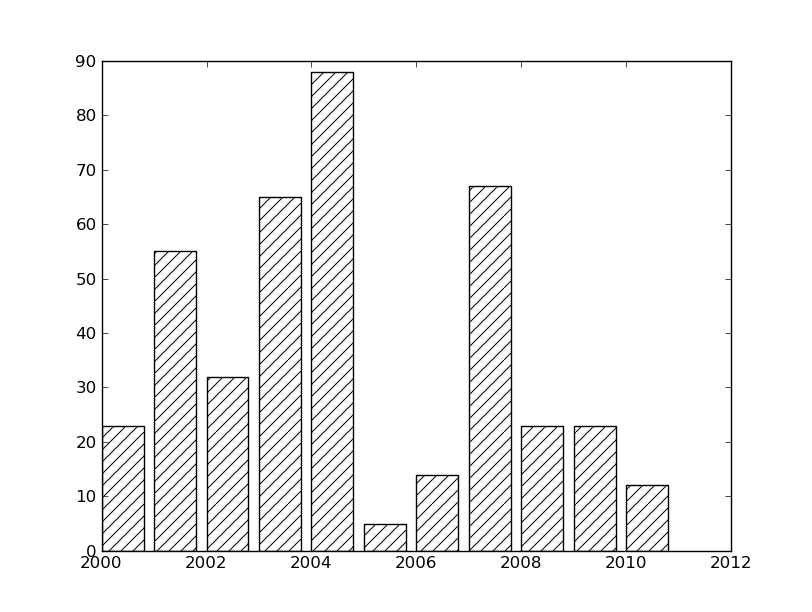
\includegraphics[scale=0.3]{bar-chart-hatch}    
    \end{center}
  \textbf{Clue} - \emph{try bar? in your ipython interpreter}
\end{frame}
\begin{frame}
\frametitle{Log-log graph}
\label{sec-16}


\begin{itemize}
\item Log-log graph
\begin{itemize}
\item 2-dimensional graph.
\item uses logarithmic scales on both axes.
\item graph appears as straight line due to non-linear scaling.
\end{itemize}
\end{itemize}
\end{frame}
\begin{frame}
\frametitle{Exercise 7:}
\label{sec-17}

  Plot a log-log chart of 
    $y = 5x^3$
  for x from 1-20.
\end{frame}
\begin{frame}[fragile]
\frametitle{\verb~loglog()~ function}
\label{sec-18}


\begin{itemize}
\item \emph{Syntax :} loglog(x, y)
\begin{itemize}
\item x, a sequence of data
\item y, a sequence of data, the same length of x
\end{itemize}
\end{itemize}
\begin{verbatim}
   In []: loglog(x, y)
\end{verbatim}
\end{frame}
\begin{frame}
\frametitle{Getting help on \verb~matplotlib~}
\label{sec-19}


\begin{itemize}
\item Help
\begin{itemize}
\item \hyperref[matplotlib.sourceforge.net--contents.html]{matplotlib.sourceforge.net/contents.html}
\end{itemize}
\item More plots
\begin{itemize}
\item \hyperref[matplotlib.sourceforge.net--users--screenshots.html]{matplotlib.sourceforge.net/users/screenshots.html}
\item \hyperref[matplotlib.sourceforge.net--gallery.html]{matplotlib.sourceforge.net/gallery.html}
\end{itemize}
\end{itemize}
\end{frame}
\begin{frame}
\frametitle{Summary}
\label{sec-20}

  In this tutorial we learnt to,
 

\begin{itemize}
\item Plot a scatter plot using ``scatter()`` function
\item Plot a pie chart using ``pie()`` function
\item Plot a bar chart using ``bar()`` function
\item Plot a log-log graph using ``loglog()`` function
\item Access the \verb~matplotlib~ online help.
\end{itemize}
\end{frame}
\begin{frame}
\frametitle{Evaluation}
\label{sec-21}


\begin{enumerate}
\item ``scatter(x, y, color='blue', marker='d')`` and ``plot(x, y,
     color='b', marker='d')`` does exactly the same.
\begin{itemize}
\item True
\item False
\end{itemize}
\item What statement can be issued to generate a bar chart with vertical
     line hatching.
\begin{itemize}
\item bar(x, y, color='w', hatch='/')
\item bar(x, y, fill=False, hatch='//')
\item bar(x, y, fill=False, hatch='|')
\item bar(x, y, color='w', hatch='\')
\end{itemize}
\end{enumerate}
\end{frame}
\begin{frame}
\frametitle{Solutions}
\label{sec-22}


\begin{enumerate}
\item False
\item bar(x, y, fill=False, hatch='|')
\end{enumerate}
\end{frame}
\begin{frame}

  \begin{block}{}
  \begin{center}
  \textcolor{blue}{\Large THANK YOU!} 
  \end{center}
  \end{block}
\begin{block}{}
  \begin{center}
    For more Information, visit our website\\
    \url{http://fossee.in/}
  \end{center}  
  \end{block}
\end{frame}

\end{document}